\chapter{颜色与吸光度}\label{ch:g11:absorbance}

一瓶运动饮料在健身房的长凳上闪着鲜亮的蓝色。它的
颜色来自溶于其中的染料，整升饮料里只有几毫克，
少得几乎无法称量，也远不足以作为固体被看见。
然而食品实验室必须检测这一含量，因为染料只能
在限量之内添加。颜色本身正是关键：溶液中
染料越多，溶液吸收的光就越多；能够测量溶液吸光多少的仪器，
实际上测得的就是浓度。

\begin{recall}
溶液的质量浓度与物质的量浓度；稀释母液；
标准溶液的标准色阶，并与未知溶液比较
（见\cref{ch:g10:concentration-and-dilution}）
\end{recall}

\begin{omfigure}
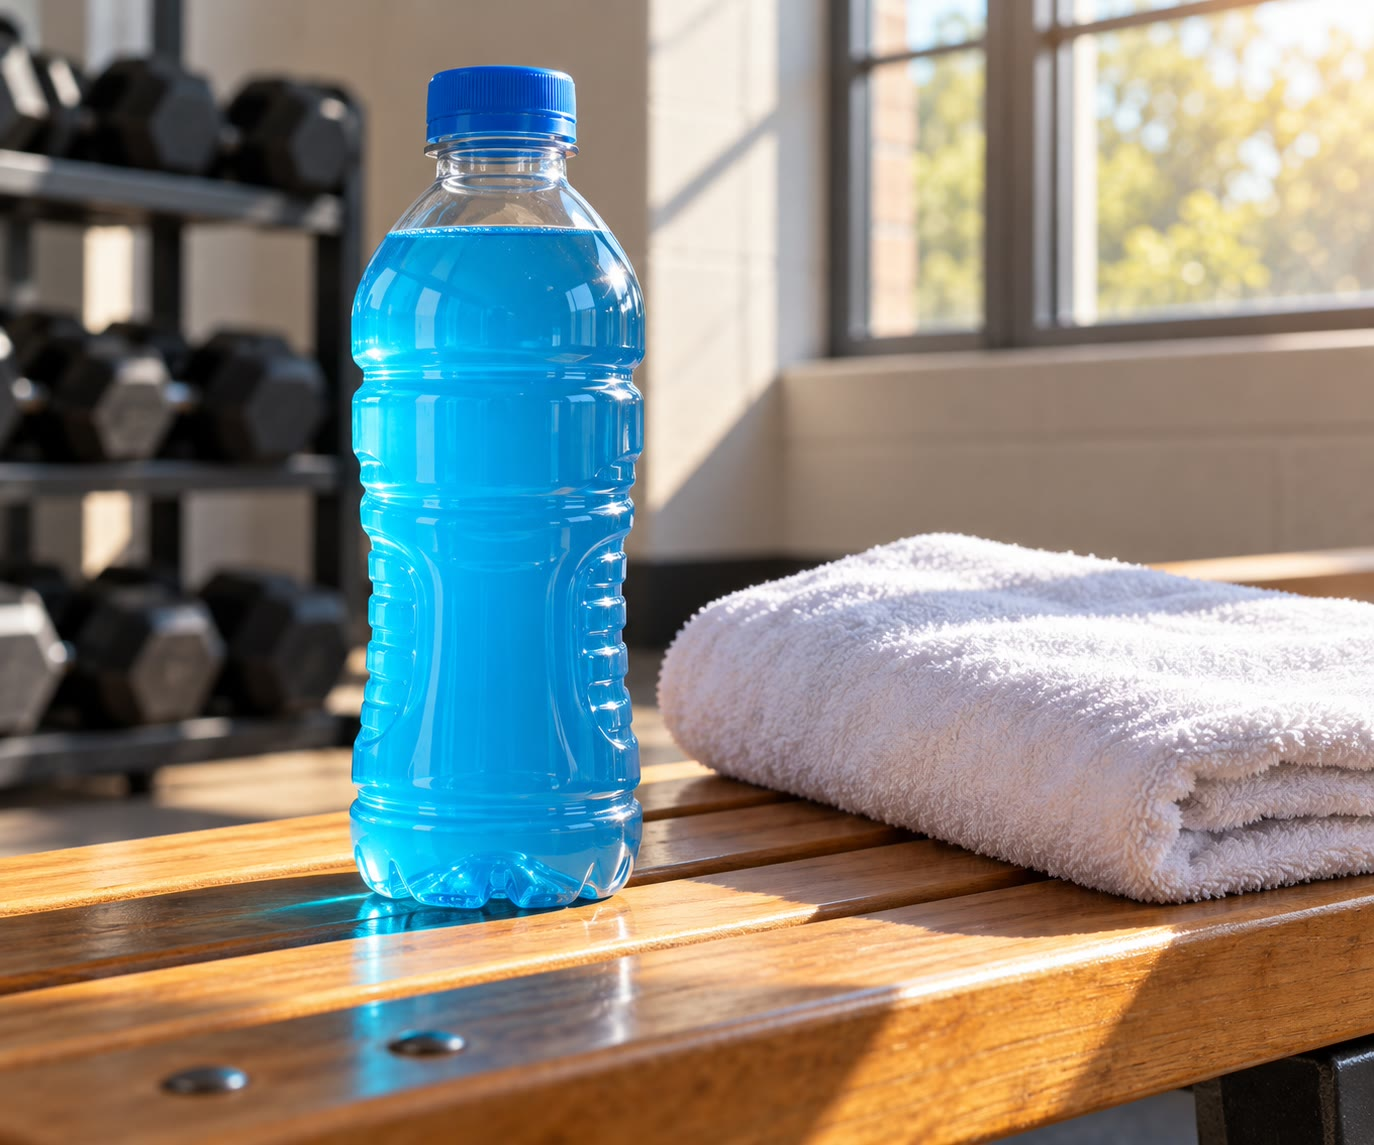
\includegraphics[width=0.5\linewidth]{images/book1/ai/g11-sports-drink.jpg}

{\small 一瓶蓝色饮料，其颜色来自每升饮料中的
几毫克染料。}
\end{omfigure}

\section{溶液的颜色}

白光（如日光）是彩虹中所有颜色的
混合。每种颜色对应一个波长，紫光约
为 \qty{400}{nm}，红光约为 \qty{750}{nm}；物理课本解释了
什么是波长，这里它只是颜色的一个标签。有色溶液会吸收
穿过它的部分光线，且对不同颜色的吸收差异很大；人眼
看到的是
透过的颜色。

\begin{definition}[互补色]\label{def:g11:absorbance:complementary}
若两种颜色混合后可得白光，则称它们为\emph{互补色}\index{互补色}。
在色轮上，互补色
彼此相对。
\end{definition}

\begin{omfigure}
\begin{tikzpicture}[font=\small]
  \foreach \a/\c/\n/\w/\t in {90/red!85!black/红/{620--750}/white,
      30/orange/橙/{590--620}/black, -30/yellow!90!orange/黄/{570--590}/black,
      -90/green!70!black/绿/{500--570}/white, -150/cyan!50!blue/蓝/{450--500}/white,
      150/violet!80!blue/紫/{400--450}/white} {
    \fill[\c] (0,0) -- (\a-30:1.8) arc[start angle=\a-30, end angle=\a+30,
      radius=1.8] -- cycle;
    \node[text=\t, font=\small\bfseries] at (\a:1.2) {\n};
    \node[font=\footnotesize, align=center] at (\a:2.45) {\w\\ nm};
  }
  \fill[white] (0,0) circle (0.45);
  \draw[<->, thick, black!70] (90:0.5) -- (-90:0.5);
  \draw[<->, thick, black!70] (30:0.5) -- (-150:0.5);
  \draw[<->, thick, black!70] (-30:0.5) -- (150:0.5);
\end{tikzpicture}

{\small 色轮，标出了近似波长。互补色
彼此相对：红色与绿色、橙色与蓝色、黄色与
紫色。}
\end{omfigure}

\begin{proposition}[看到的颜色]\label{prop:g11:absorbance:colour-seen}
若某溶液主要吸收白光中的某一种颜色，
则它呈现的颜色是与之互补的颜色。
\end{proposition}

\begin{proof}
在本阶段不加证明地承认：透过的光是白光减去被吸收的
那种颜色后的剩余光，人眼将其看作互补色。
\end{proof}

\begin{example}[两种食品染料]\label{ex:g11:absorbance:dyes}
% ledger: lmax:E133, lmax:E102
运动饮料中的蓝色染料即亮蓝（E133），
主要吸收橙红色光，波长约为 \qty{629}{nm}，因此呈现蓝色。
黄色染料柠檬黄（E102）主要吸收紫蓝色光，波长约为
\qty{427}{nm}，因此呈现黄色。绿色饮料通常两者都含有。
\end{example}

\section{吸收光谱}

\begin{definition}[吸收光谱]\label{def:g11:absorbance:spectrum}
溶液的\emph{吸收光谱}\index{吸收光谱}是
溶液所吸收的光（即其吸光度，定义见下一节）
随波长变化的图像。使吸收最大的
波长记为 $\lambda_{\max}$。
\end{definition}

\begin{omfigure}
\begin{tikzpicture}
\begin{axis}[width=0.85\linewidth, height=6cm, xmin=380, xmax=750,
    ymin=0, ymax=0.95, xlabel={波长 $\lambda$ (\si{nm})},
    ylabel={吸光度 $A$}, axis lines*=left, ymajorgrids,
    grid style={gray!20}, tick label style={font=\small},
    label style={font=\small}, xtick={400,450,500,550,600,650,700,750},
    ]
  % ledger: lmax:E133, abs:E133, lmax:E102, abs:E102 (band shapes synthetic)
  \addplot[very thick, cyan!60!blue] table[x=lambda, y=E133]
    {figdata/out/grade-11-absorbance-a.dat};
  \addplot[very thick, orange!85!yellow] table[x=lambda, y=E102]
    {figdata/out/grade-11-absorbance-a.dat};
  \node[font=\small, align=left, anchor=west, text=cyan!60!blue!80!black]
    at (axis cs:668,0.62) {蓝色染料 E133,\\ \qty{5.0}{mg/L}};
  \node[font=\small, align=left, anchor=west, text=orange!80!black]
    at (axis cs:470,0.66) {黄色染料 E102,\\ \qty{15}{mg/L}};
  \addplot[dashed, black!50] coordinates {(629,0) (629,0.82)};
  \addplot[dashed, black!50] coordinates {(427,0) (427,0.795)};
  \node[font=\small, anchor=south] at (axis cs:629,0.83) {\qty{629}{nm}};
  \node[font=\small, anchor=south] at (axis cs:427,0.81) {\qty{427}{nm}};
\end{axis}
\end{tikzpicture}

{\small 两种染料在水中的吸收光谱，装在
\qty{1}{cm}厚的比色皿中。谱带形状由一个简单模型画出；
吸收峰的位置及其高度取自两种染料的
技术指标。}
\end{omfigure}

\begin{remark}[读懂光谱]\label{rem:g11:absorbance:reading}
蓝色染料在\qty{520}{nm}以下几乎不吸光：蓝光和紫光
可以透过，溶液呈蓝色。黄色染料在
\qty{520}{nm}以上几乎不吸光：绿光、黄光、橙光和红光
都可以透过，人眼看到黄色。在\qty{629}{nm}处
只有蓝色染料吸光；在\qty{427}{nm}处，几乎只有黄色染料吸光。
\end{remark}

\section{吸光度与分光光度计}

\begin{definition}[吸光度]\label{def:g11:absorbance:absorbance}
溶液在选定波长下的\emph{吸光度}\index{吸光度} $A$，
是分光光度计显示的数值，用于测量溶液对该波长光的
吸收程度。吸光度没有单位；
纯溶剂的吸光度为零，
吸光度越大，溶液吸收的光越多。
\end{definition}

\begin{omfigure}
\begin{tikzpicture}[font=\small]
  % lamp
  \shade[ball color=yellow!40] (0,0.6) circle (0.32);
  \foreach \a in {0,45,90,135,180,225,270,315} \draw[yellow!60!orange, thick] (\a:0.4) ++(0,0.6) -- ++(\a:0.18);
  \node[anchor=north] at (0,-0.25) {灯};
  \draw[black!60, thick] (0.8,0.6) -- (1.75,0.6);
  % prism
  \fill[cyan!10, draw=black!60] (1.75,0.15) -- (2.55,0.15) -- (2.15,1.15) -- cycle;
  \node[anchor=north] at (2.15,-0.25) {棱镜};
  \foreach \c/\d in {violet/0.35, blue/0.22, green!70!black/0.08, yellow!90!orange/-0.06,
      orange/-0.2, red/-0.34}
    \draw[\c, thick] (2.45,0.6) -- (3.45,{0.6+\d});
  % slit
  \fill[black!70] (3.5,0.92) rectangle (3.6,1.4);
  \fill[black!70] (3.5,-0.2) rectangle (3.6,0.52);
  \node[anchor=north] at (3.55,-0.25) {狭缝};
  \draw[orange, very thick] (3.6,0.6) -- (4.75,0.6);
  % cuvette
  \pic (cv) at (5,0) {cuvette={0.75}{cyan!50!blue!45}};
  \node[anchor=north] at (5,-0.25) {比色皿};
  \draw[orange!60, thick] (5.3,0.6) -- (6.3,0.6);
  % detector and display
  \fill[black!15, draw=black!60] (6.3,0.2) rectangle (6.9,1.0);
  \node[anchor=north] at (6.6,-0.25) {探测器};
  \draw[black!60] (6.9,0.6) -- (7.4,0.6);
  \fill[black!80, draw=black] (7.4,0.25) rectangle (9.4,0.95);
  \node[green!70!white, font=\footnotesize\ttfamily] at (8.4,0.6) {A = 0.590};
  \node[anchor=north] at (8.4,-0.25) {显示屏};
\end{tikzpicture}

{\small 分光光度计的原理。棱镜把白光分散成
各种颜色；狭缝只让一种波长的光通过，波长由
用户选定；探测器比较离开比色皿的光与
进入比色皿的光，显示屏给出吸光度。}
\end{omfigure}

\begin{remark}[数值从何而来]\label{rem:g11:absorbance:log}
吸光度由仪器根据射入和射出溶液的光的
强度计算得出，计算用到一个数学函数，
即中学最后一年学过的对数。大学教材会
给出公式；这里，吸光度就是仪器所
读出的数值。
\end{remark}

\begin{inthelab}[分光光度计调零]
比色皿、溶剂和仪器本身都会吸收少量光。
测量之前，先将装有纯溶剂的比色皿，即
\emph{空白}放入仪器中，仪器调节为在选定波长处读数为
$A = 0$，之后的每次读数都是
仅由溶质引起的吸光度。比色皿应始终手持
磨砂面，并擦拭干净：透明面上的指纹
也会吸收光。
\end{inthelab}

\begin{omfigure}
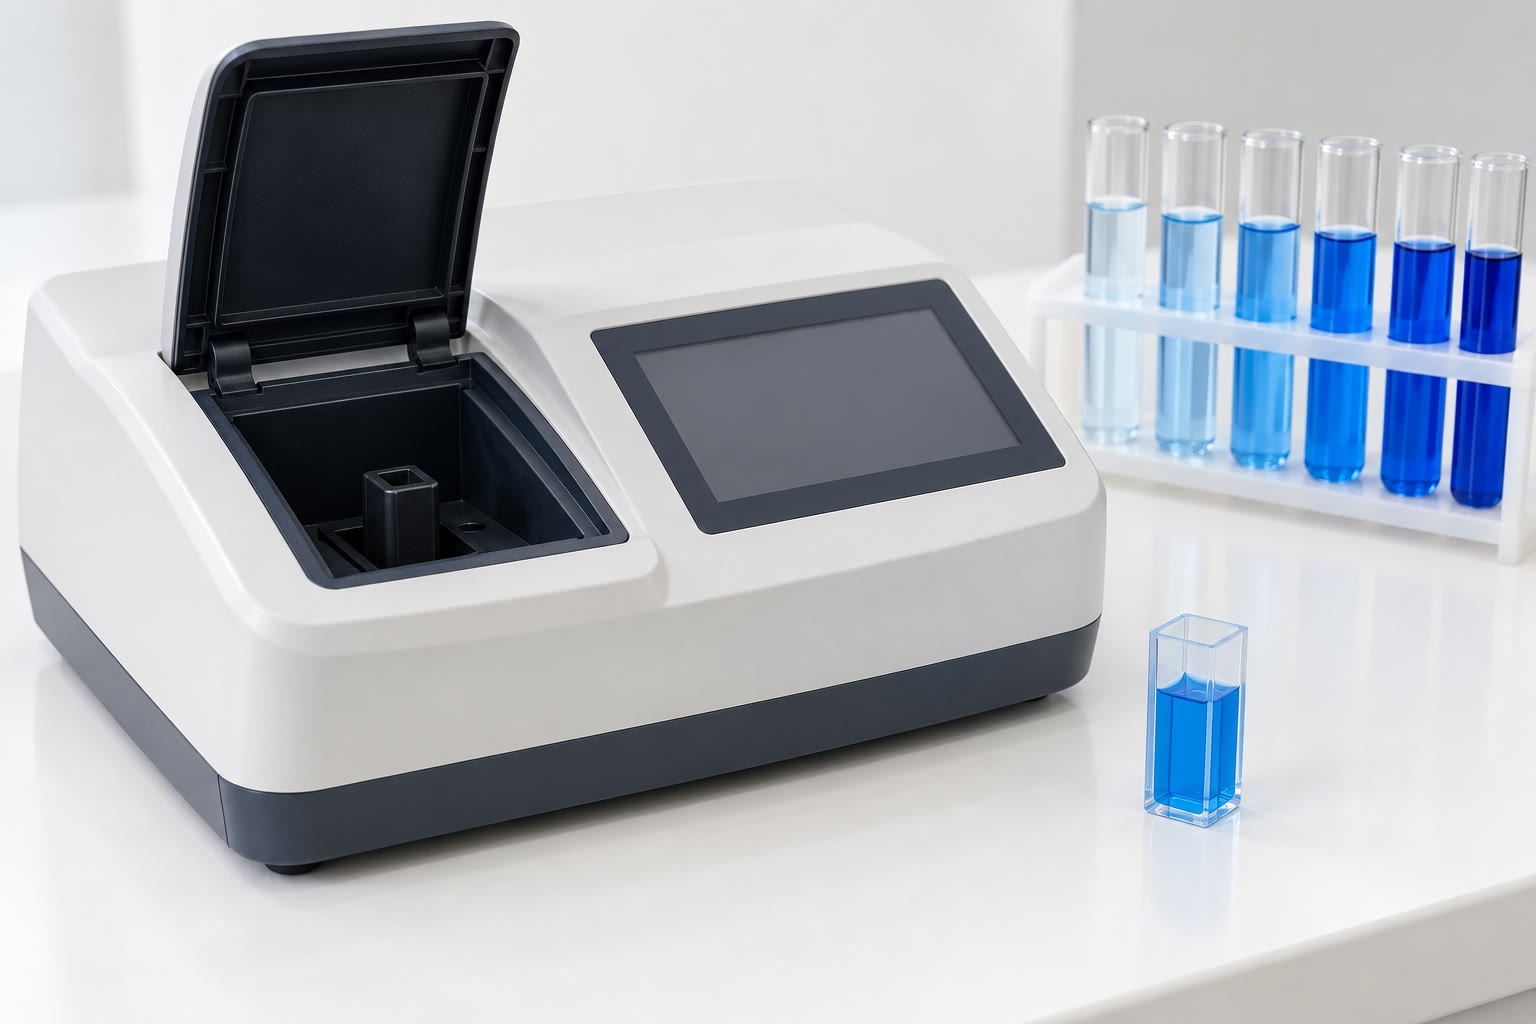
\includegraphics[width=0.5\linewidth]{images/book1/ai/g11-spectrophotometer.jpg}

{\small 分光光度计及其方形比色皿。}
\end{omfigure}

\section{比尔–朗伯定律}

\begin{definition}[摩尔吸收系数]\label{def:g11:absorbance:epsilon}
称溶解物种在给定波长下的\emph{摩尔吸收系数}\index{摩尔吸收系数}
$\varepsilon$ 表示一摩尔该物种吸收光的
能力强弱；它
取决于物种、溶剂和波长，单位以
\si{L/(mol.cm)}表示。
\end{definition}

\begin{proposition}[比尔–朗伯定律]\label{prop:g11:absorbance:beer-lambert}
对于仅含一种吸光物种的稀溶液，其
物质的量浓度为 $c$，比色皿厚度为 $\ell$，则
在给定波长下的吸光度为
\[
  A = \varepsilon\, \ell\, c .
\]
吸光度与浓度成正比。
\end{proposition}

\begin{proof}
在本阶段不加证明地承认，证明见大学教材。
\end{proof}


\begin{remark}[以质量浓度表示]\label{rem:g11:absorbance:mass}
% ledger: abs:E133, mw:E133
由于 $c = C_m / M$，定律也可写作 $A = a\, \ell\, C_m$，
其中 $a = \varepsilon / M$，单位为 \si{L/(g.cm)}。食品
染料的规格给出 $a$：对蓝色染料 E133，在 \qty{629}{nm} 波长下，$a =
\qty{164}{L/(g.cm)}$，其摩尔质量为 \qty{792.9}{g/mol}，
则 $\varepsilon = 164 \times 792.9 = \qty{1.30e5}{L/(mol.cm)}$。该染料浓度仅为
\qty{5.0}{mg/L} 的溶液，置于 \qty{1}{cm} 的比色皿中，
即可读得 $A = 164 \times 1 \times 0.0050 = 0.82$。
\end{remark}

\begin{remark}[仅适用于稀溶液]\label{rem:g11:absorbance:dilute}
该正比关系仅对稀溶液成立，实际中
通常要求普通仪器上吸光度在 1 至 1.5 左右以下。浓度过高的溶液
须先以已知倍数稀释，
再进行测量。
\end{remark}

\section{测定浓度}

\begin{definition}[标准曲线]\label{def:g11:absorbance:calibration-line}
称\emph{标准曲线}\index{标准曲线}为同一种物质的一系列标准溶液
在相同波长、同一比色皿中测得的吸光度，
对其浓度作出的图像。当比尔–朗伯定律成立时，
它是一条过原点的直线。
\end{definition}

\begin{method}[用标准曲线测定浓度]\label{met:g11:absorbance:calibration}
\begin{enumerate}
  \item 记录该物质的吸收光谱，并选择
        波长 $\lambda_{\max}$，该处吸光度最大，
        且波长有微小误差时吸光度变化最小。
  \item 用空白溶液将仪器调零。
  \item 将母液稀释，配制标准溶液，
        并测定其吸光度。
  \item 以 $A$ 对浓度作图，并画出
        过原点且最接近各数据点的直线。
  \item 测定未知溶液，必要时先稀释，使其吸光度
        落在标准溶液的吸光度范围之内，并从直线上读出其浓度
        （或将 $A$ 除以斜率），再乘以
        稀释倍数。
\end{enumerate}
\end{method}

\begin{omfigure}
\begin{tikzpicture}
\begin{axis}[width=0.72\linewidth, height=6cm, xmin=0, xmax=5.6,
    ymin=0, ymax=0.95, xlabel={E133 的浓度（\si{mg/L}）},
    ylabel={\qty{629}{nm} 处的吸光度}, axis lines*=left, ymajorgrids,
    xmajorgrids, grid style={gray!20}, tick label style={font=\small},
    label style={font=\small}]
  % ledger: abs:E133 (points synthetic: exact values + fixed offsets)
  \addplot[only marks, mark=*, mark size=2.2pt, omDef] table[x=C, y=A]
    {figdata/out/grade-11-absorbance-b.dat};
  \addplot[thick, omProp, domain=0:5.5] {0.164*x};
  \addplot[dashed, black!60] coordinates {(0,0.590) (3.6,0.590) (3.6,0)};
  \node[font=\small, anchor=south west] at (axis cs:0.1,0.6) {未知：$A = 0.590$};
  \node[font=\small, anchor=west] at (axis cs:3.65,0.22) {\qty{3.6}{mg/L}};
\end{axis}
\end{tikzpicture}

{\small 蓝色染料的标准曲线：五个标准溶液（数据点）及
过原点的直线，斜率为 \qty{0.164}{L/mg}。未知溶液的
吸光度读数 $A = 0.590$，其浓度为 $0.590 / 0.164 =
\qty{3.6}{mg/L}$。}
\end{omfigure}

\begin{example}[五个标准溶液]\label{ex:g11:absorbance:standards}
取浓度为 \qty{100}{mg/L} 的蓝色染料母液，稀释配制
每份 \qty{100.0}{mL} 的标准溶液。对于 \qty{2.0}{mg/L} 的溶液，
稀释倍数为 50，故取 \qty{2.0}{mL} 母液，定容至 \qty{100.0}{mL}。
五个标准溶液的浓度由 1 至 \qty{5}{mg/L}，读数分别为 0.168、0.325、0.494，
0.652 和 0.823，与 $0.164 \times C$ 的偏差在千分之几以内，
基本落在图中的直线上。
\end{example}

\section{练习}

\begin{exercise}[$\star$]\label{exo:g11:absorbance:1}
某溶液主要吸收橙色光，它呈现什么颜色？
若另一溶液主要吸收紫色光，它又呈现什么颜色？
\end{exercise}

\begin{exercise}[$\star$]\label{exo:g11:absorbance:2}
利用色轮，写出绿色溶液主要吸收的颜色，
并给出该颜色所覆盖的波长范围。
\end{exercise}

\begin{exercise}[$\star$]\label{exo:g11:absorbance:3}
从吸收光谱上读出各染料的波长 $\lambda_{\max}$，
以及该波长处的吸光度。
\end{exercise}

\begin{exercise}[$\star$]\label{exo:g11:absorbance:4}
某染料溶液浓度为 \qty{2.0}{mg/L}，读数为 $A = 0.30$。
同一染料浓度为 \qty{6.0}{mg/L} 的溶液，在相同比色皿、相同波长下，
读数应为多少？浓度为 \qty{1.0}{mg/L} 时又为多少？
\end{exercise}

\begin{exercise}[$\star$]\label{exo:g11:absorbance:5}
分光光度计的空白是什么，
为何要用它将仪器调零？
\end{exercise}

\begin{exercise}[$\star\star$]\label{exo:g11:absorbance:6}
利用蓝色染料的标准曲线，求出
读数为 $A = 0.41$ 的溶液的浓度。
\end{exercise}

\begin{exercise}[$\star\star$]\label{exo:g11:absorbance:7}
测定蓝色染料时，为何将分光光度计设置在
\qty{629}{nm} 而不是 \qty{550}{nm}？请给出两个理由。
\end{exercise}

\begin{exercise}[$\star\star$]\label{exo:g11:absorbance:8}
将未稀释的饮料在 \qty{629}{nm} 处测得 $A = 2.4$，读数过高，
不可信。将其稀释五倍后，读数为 $A = 0.48$。求饮料中
蓝色染料的浓度。
\end{exercise}

\begin{exercise}[$\star\star$]\label{exo:g11:absorbance:9}
% ledger: mw:E102, abs:E102
柠檬黄溶液的浓度为 \qty{15.0}{mg/L}，在
\qty{427}{nm} 处，用 \qty{1.00}{cm} 比色皿测得 $A = 0.795$。计算其吸收率 $a$，单位为
\si{L/(g.cm)}，再求其摩尔吸光系数（摩尔质量为
\qty{534.4}{g/mol}）。
\end{exercise}

\begin{exercise}[$\star\star$]\label{exo:g11:absorbance:10}
观察两种染料的光谱，黄色染料在哪一波长以上
几乎不吸收光？为何即使绿色饮料中还含有黄色染料，
仍可在 \qty{629}{nm} 处测定蓝色染料？
\end{exercise}

\begin{exercise}[$\star\star$]\label{exo:g11:absorbance:11}
同一溶液改用厚度为 \qty{2.0}{cm} 的比色皿测量，
而不是 \qty{1.0}{cm}。其吸光度如何变化？为什么？
\end{exercise}

\begin{exercise}[$\star\star\star$]\label{exo:g11:absorbance:12}
蓝色染料标准溶液的浓度分别为 5、10、20 和 \qty{40}{mg/L}，读数分别为 0.82、1.62、
2.30 和 2.70。求各自的 $A / C$，你发现了什么？
哪些标准溶液可用于绘制标准曲线，对
读数为 $2.5$ 的未知样品应如何处理？
\end{exercise}

\begin{exercise}[$\star\star\star$]\label{exo:g11:absorbance:13}
一瓶绿色饮料同时含有蓝色染料和黄色染料。在
\qty{1.00}{cm} 比色皿中，测得 \qty{629}{nm} 处 $A = 0.574$，
在 \qty{427}{nm} 处 $A = 0.53$。已知蓝色染料在该波长处几乎不吸收光，
而黄色染料在 \qty{629}{nm} 处不吸收光。求两种染料的质量
浓度（取 $a = \qty{164}{L/(g.cm)}$ 与
$a = \qty{53.0}{L/(g.cm)}$）。
\end{exercise}

\begin{exercise}[$\star\star\star$]\label{exo:g11:absorbance:14}
某学生忘了做空白对照，用空比色皿将仪器调至零点，
此后每个读数都偏高 \num{0.040}。未知样品读数为
$0.368$，她用真实标准曲线的斜率 $0.164$ 去除读数，
得到的浓度是多少？真实浓度是多少？她的结果
偏差了百分之几？
\end{exercise}

\begin{exercise}[$\star\star\star$]\label{exo:g11:absorbance:15}
% ledger: adi:E102
柠檬黄的每日允许摄入量为每千克
体重 \qty{10}{mg}。某饮料中含柠檬黄 \qty{20}{mg/L}。
需饮用多少体积的该饮料，才能使 \qty{60}{kg} 成年人一天的摄入量恰好达到此限量？
这一风险是否现实？
\end{exercise}

\section{问题：运动饮料的蓝色}


\begin{problem}[{周末问题——一个孩子需要喝掉多少瓶蓝色运动饮料，
才能达到其色素的安全
每日限量？}]
\label{pb:g11:absorbance:1}
% ledger: lmax:E133, abs:E133, mw:E133, adi:E133
某食品实验室检测一种运动饮料中的蓝色染料 E133，该饮料以
\qty{500}{mL} 瓶装出售。染料的技术指标给出其摩尔质量
为 \qty{792.9}{g/mol}，其每日允许摄入量为每千克
体重每天 \qty{6}{mg}，此量可终生每天食用，
不会带来明显风险。

\medskip
\noindent\textbf{第一部分——颜色与光谱。}
\begin{enumerate}
  \item 该饮料呈蓝色。借助色轮，它吸收最多的是哪一种
        颜色的光？
  \item 在光谱上读出染料的 $\lambda_{\max}$。
  \item 为何染料在 \qty{450}{nm} 处的吸光度几乎为零？
        这与其颜色一致吗？
  \item 测量应在哪一波长下进行？
\end{enumerate}

\medskip
\noindent\textbf{第二部分——标准曲线。}
\begin{enumerate}[resume]
  \item 将 \qty{50.0}{mg} 纯染料溶解，配成 \qty{500.0}{mL}
        母液。计算其质量浓度，单位为 \si{mg/L}。
  \item 配制浓度分别为 1.0、2.0、3.0、4.0 和 \qty{5.0}{mg/L} 的标准溶液，
        每种各 \qty{100.0}{mL}。配制 \qty{3.0}{mg/L} 标准溶液
        需要多少体积的母液？需用哪种玻璃仪器？
  \item 这些标准溶液的读数分别为 0.168、0.325、0.494、0.652 和 0.823。求
        各自的 $A / C$，并说明这些点近似落在一条过原点、斜率约为
        \qty{0.164}{L/mg} 的直线上。
  \item 为何该直线必须过原点？
  \item 由此推出该染料的吸收率 $a$，单位为 \si{L/(g.cm)}（比色皿厚
        \qty{1.00}{cm}），再求其摩尔吸光系数。
\end{enumerate}

\medskip
\noindent\textbf{第三部分——饮料。}
\begin{enumerate}[resume]
  \item 取 \qty{25.0}{mL} 饮料，加水稀释至 \qty{50.0}{mL}。
        稀释倍数为多少？
  \item 稀释后的饮料读数为 $A = 0.590$。求其中
        染料的浓度。
  \item 推出饮料本身的染料浓度。
  \item 未稀释的饮料读数应为多少？为何要稀释？
  \item 计算一瓶饮料中染料的质量。
  \item 计算一瓶饮料中染料的物质的量（以摩尔表示）。
\end{enumerate}

\medskip
\noindent\textbf{第四部分——每日允许摄入量。}
\begin{enumerate}[resume]
  \item 体重为 \qty{30}{kg} 的儿童，每天
        可摄入多少质量的染料？
  \item 该儿童一天需喝下多少瓶饮料，
        才能达到此限量？
  \item 这相当于多少体积的饮料？请加以评述。
  \item 对体重为 \qty{70}{kg} 的成年人，提出同样的问题。
  \item 给出最终答案：一个 \qty{30}{kg} 的儿童一天
        需喝下多少瓶 \qty{500}{mL} 的饮料，
        才能达到染料的每日允许摄入量？
\end{enumerate}
\end{problem}
